\chapter{科学的推論}
科学におけるモデルおよび、数理統計学におけるモデルについて説明し、その違いを明らかにする。


\section{モデル}
モデル(模型)とは、現実を表していると思わせるような、作られたものであり、次の特徴を備えています。
\begin{enumerate}
    \item モデルは本物の特徴の一部を推測可能。本物との乖離の程度も推測できる
    \item (1)を行うために、複数の仮定により構築される。また、それらの仮定は、現状の知識では明らかではないまたは、現実的には成立していないことがある。
    %推測可能なことを増やすために仮定を増やすことがある。
    % \item モデルは本物の要素・特徴の全体を推測することはできない。
    \item モデルは間違った推測をする。
\end{enumerate}
  
例えば、車のプラモデルはモデルの一つです。本物の特徴の一つである大きさを推測可能にするため、スケール(例えば、1/24など)を決めて作られている。ドアや車体の幅を計測し、スケール倍すれば、本物の大きさを推測できる。普段長さを測れない場所であっても、手のひらに収まるプラモデルであれば、どの部分でも推測が可能になる。言い換えれば、本物の車がなくても、スケールを維持した車のプラモデルを持っていれば、簡単に大きさに関する推測が可能になる。



\if 0
モデルの仮定によって推測可能なことが増えることがある。
例えば、本物のパーツの重量に応じて、モデルのパーツの重さを変化させる。
こうすることで、プラスティックでできたモデルの重さを計測すると、そこから本物の重さの推測が可能になる。
他にも推測したいこと、例えば、素材の質感や色や重量、または車の速度といった特徴なども、モデルに仮定を追加することで、本物の様子を捉えることが可能になっていく。
\fi

本物の車を持って来れば、本物の様子を推測することが可能であるので、本物の車は、車自身のモデルということができるが、車を車自身のモデルとすると、それまであった利便性が損なわれる。
%また、モデルの仮定を増やせば、本物の車にモデルを近づけることが可能である。
おおよその車体の長さが知りたいのに、わざわざ長い測りが必要になることや、手に持って観察することもできない。
このように、細部まで推測可能にするというのは、デメリットになることがあり、モデルとして利用することはない。

細部まで推測可能なモデルは使うことは稀であり、車のモデルとして、大きさの尺度を保っていない直方体のブロックを使うことがある。このモデルでも推測できることがある。3台の同じ車を縦列駐車するのに必要な長さなどは、直方体三つ分と推測が可能である。
モデルの作り込みの程度によって推測できることは様々である。
%が異なる。統計学を利用するときは、目的について考えることは少なく、儀式的に採用した手順に従うことが多い。

真球を車のモデルし、車の大きさに関する推測を行うと、現実の大きさと推測は大きく乖離することが考えられる。
モデルが本物の推測に使えないということに判断を下すには、本物のデータとモデルの出す推測を複数の指標から比較し考察することになる。

%車のモデルという題材からモデルの特徴を挙げた

モデルは本物ではないが、推測に役にたつ物として利用する。モデルと本物が極めて一致するように感じられることもあると思うが、モデルは本物ではない。



\section{統計モデル}
統計モデルについて説明し、モデルを使って現実を推測することを概念図を用いて説明する。まず、統計モデルは、数理統計の知識を使いモデルを構築され、現実を推測するために用いられる。簡単な統計モデルを例に挙げると、次のような仮説から構築される。

\begin{enumerate}
    \item (仮定1)確率変数が同一の分布から独立に得られる(i.i.d)
    \item (仮定2)その分布関数は、$f(x)$と書ける。
    \item (仮定3)分布関数の母数に関する仮説\footnote{三番目の仮説のみを統計モデルと主張する流派もある\cite{塩見_正衛2021}}
\end{enumerate}

統計モデルにより推定したい対象またはデータが、統計モデルの仮定から外れていることは多々ある。
まず仮定1、独立性と同一の分布という仮定は、数学的厳密な定義がある。
科学におけるその意味を考えることで、その仮定が現実の世界において当てはまらないことがわかる。
まず、各変数が独立とは、得られたデータに相関が全くないこと考えられ、それは科学においては当てはまっていないことの方が多い。例えば、人の身長を計測器により繰り返し観測すると、その計測器や扱う人の癖がデータに含まれ、それはデータの傾向を決定する因子となり、相関があると考えられる。
もし、相関がない計測状況が設定できたとしても、人の身長はその背景にある社会や遺伝的な繋がりが因子となっており、相関が無いと言い切ることは難しい。
同一の分布とは、同一の数学的規則に自然が支配されていることを仮定していると考えられ、サイコロやコインのトスではそのように考えても矛盾しない。人の身長は、母父の大きさや成長過程における栄養の量などの因子によって成長すると考えることは科学的ではあるが、サイコロをふって決定されていると考えるのは妥当とは言い切れない\footnote{そう考えてもいい}。
仮定が科学において妥当とは言い切れないモデルを使って推測を行うことになる。
%統計モデルの数学的な仮定が科学と対応しているとは言い難い。

以下では、統計モデルを$M(\bm{a})$とし、ここで$\bm{a}$は、仮定3の統計モデルの母数であり、母数が複数あることも考慮し、ベクトルで表記しておく。

\begin{SMbox}{学問間に生じているモデルに関する認識の違い}
モデルが本物であるか否かは、学問領域によって認識が異なっている。
生物物理学の視点では、モデルは現実を推測するための偽物のことだと考えていることの方が多い。
モデルが自分の知りたいことをうまく予測してくれさえいればいいという立場である。
一方で、数学では、モデルを現実と捉える傾向がある。モデルにより世界が支配されていると考えているのである。例えば、ある数学者は、流体モデルに解が安定的に存在するかがわからないから飛行機に乗りたくないと思っていると言う雰囲気がある。
現代の統計学はどちらかと言うと数学者が作った枠組みを統計ユーザーが受け入れてしまったため、ユーザーたちは、数学者のように世界を捉ようとしているように見える。
\end{SMbox}


\if 0
\begin{mybox}
    %\begin{quotation}
    \paragraph{頻度主義・ベイズ主義}
    頻度主義・ベイズ主義は統計学の流派を表す言葉である。頻度主義者であると言う人はあまり見たことがないが、ベイズ主義者はよく見る。ベイズ主義者は頻度主義者を非難するような主張をすることが多々ある。それぞれの立場を正確に説明した文献がないので、何を意味しているのかを私は理解できていない。

    おそらく、頻度主義では、モデルと母集団を一致させて考えており、このことを念頭にすれば頻度主義的な議論が理解できると思う。この立場にたてば、中心極限定理がデータにも適応可能になり、あらゆるデータが正規分布で推定可能にることを主張できる\footnote{本当にそう考えているのか確信が持てない}。
    %\end{quotation}
\end{mybox}
\fi


\if 0
\begin{brokenbox}[colback=yellow]
    \blindtext[5]
  \end{brokenbox}
\fi 
\subsection{数理モデルの機能}
数理モデルには予測・サンプリングという機能がある。それぞれ説明していく。
\paragraph{予測}

次に説明するサンプリングを使うことで出現しやすい場所を数値的に計算することが必要となるモデルもある。

\paragraph{サンプリング}
サンプリングは、モデルを使ってデータを生成する方法である。モデルが説明したいデータの出現頻度をよく予測できるなら、モデルが生成したデータは実際に得られるデータと似たものになる。

\section{数理統計学におけるモデル}
数理統計学は、モデルが生成した有限個の確率変数からモデルの母数を推測する方法論を提供している。



\if 0
\subsubsection{オッカムの剃刀}

仮定の追加には合理的な理由が必要だと考えられます\footnote{仮定を追加した統計モデルはベイズ統計と書かれた本で学ことができます。}。

\begin{figure}
    \begin{center}
%\includesvg{../markdown/section1/statistics_model.svg}
\end{center}
\end{figure}
\fi
\section{統計学の用語}

\subsection{母集団、無作為抽出、サンプリング}
母集団は興味のある対象全体の集団のことである。例えば、17歳男性の身長に関心があるならば、17歳男性の全員の集合が母集団である。
無作為抽出とは、偏りなく母集団からデータを取得することである。
無作為抽出することで、都合の良い結果が集まらないようにしている\footnote{無作為抽出しなければならないのはモデルの仮定1を満たすためだという主張を見かけたことがある(文献を探すべき)。モデルの仮定を現実が満たすようにすることは難しいので、そのように考えなくて良い。}。
サンプリングは無作為抽出の英訳である。本書では、モデルからの無作為抽出のことをあえてサンプリングとカタカナで記述し、現実の作業である無作為抽出と区別をする。この使い分けは一般的でない。

\subsection{標本、サンプルサイズ、標本数}
\begin{defi}
母集団から無作為抽出して得た標本に含まれるデータの個数をサンプルサイズ(標本の大きさ)といい、その数を$T$や$n$で表す。同じ実験を繰り返して行ない、複数の標本を作ると、その標本の個数を標本数という。
モデルからサンプリングした場合も、その確率変数の集まりを標本という。
モデルの標本において、標本の大きさが大きいものを大標本、小さいものを小標本と言う。
\end{defi}
例えば、無作為抽出しデータを$20$個得る実験を30回繰り返した場合、サンプルサイズ$20$の標本を$30$得たことになる。言い換えれば、標本数$30$で、サンプルサイズは$20$であると言う。

サンプルサイズを標本数と言う流儀の学問もあるようなので注意が必要である
\footnote{業界によって様々な慣習があり(\url{https://biolab.sakura.ne.jp/sample-size.html})、業界の慣習に(師匠の言うことに)従った方が余計なトラブルを減らせると考えられる(\url{https://www.jil.go.jp/column/bn/colum005.html})。この言葉くらいは統一して記述したい。本書でも途中で間違った使い方をしてしまうかもしれないが、なるべく間違わないようにしたい}。


\section{モデルを使った推測}
d

\begin{figure}
    \begin{center}
        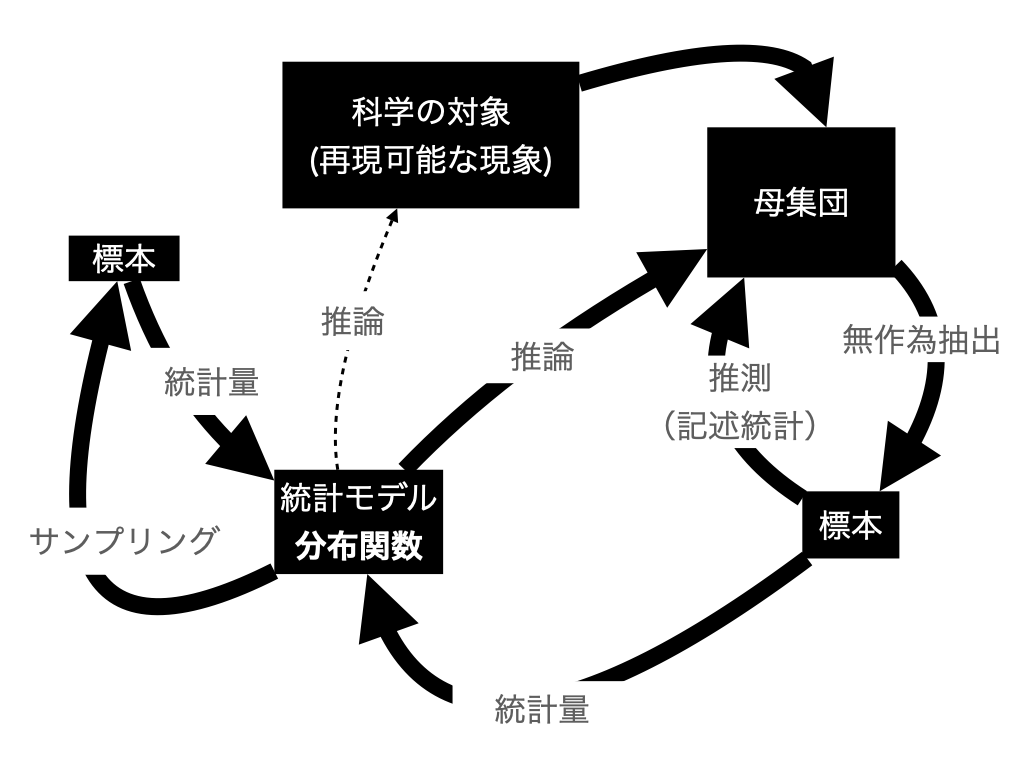
\includegraphics[width=15cm]{./image/01_/conceptual_diagram/conceptual_diagram.002.png}
        \caption{統計モデルによる現象の推測に関する概念図}
        \label{fig:conceptual_diagram_statistics}
    \end{center}
\end{figure}
    

